\documentclass[12pt,a4paper]{article}

% Данные для титульной страницы

% Номер лабораторной работы
\newcommand{\labnumber}{9}

% Название работы
\newcommand{\labtitle}{Строки в языке СИ}

% Группа студента
\newcommand{\group}{ПО-4}

% Студент, выполнивший работу
\newcommand{\labauthor}{Галанин П. И.}

% Должность преподавателя
\newcommand{\teacherstatus}{ст. преподаватель}

% Преподаватель
\newcommand{\teacher}{Хацкевич М. В.}

% Дата
\newcommand{\labdate}{2020}

% Подключение стилевого файла
\usepackage{../labwork} 

% Используемые языки программирования в исходниках в отчете
\lstloadlanguages{C}



\begin{document}



% Добавляем титульный лист
\maketitle



% Заголовок
\labheading



% Цель работы
\begin{labgoal}
Изученить принципы обработки строк в языке Си: ввод-вывод строк, использование стандартных функций языка С, работа с памятью.
\end{labgoal}



% Метка начала отчета по работе
\labreport

\begin{conductionA14}
Условие: Дана строка, содержащая полное имя файла, то есть имя диска, список
каталогов (путь), собственно имя и расширение. Выделить из этой строки имя
файла, а по расширению определить, что это за файл (например: «exe» -
исполняемый, «gif», «jpg» - графический, «doc» - текстовый документ и т.д.).
\end{conductionA14}



Исходный код программы изображен на листинге \ref{lst:lab9-a14}.



\lstinputlisting[
  language=C,
  caption={Task A 14},
  label={lst:lab9-a14}
]{a14.c}



Вывод программы при jpg-файле на рисунке \ref{fig:a14-jpg}.



% Вставляем изображение
\begin{figure}[ht]
  \centering
  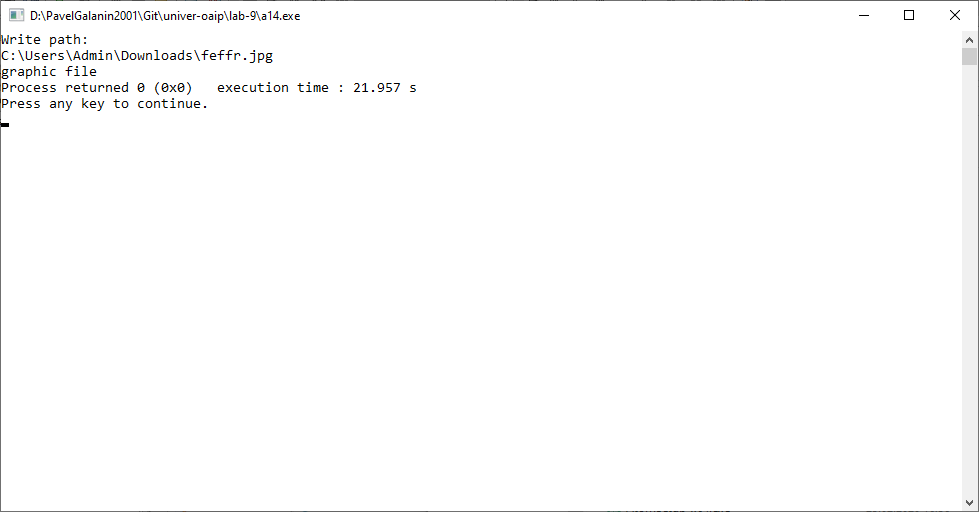
\includegraphics[width=5cm]{imgs/a14jpg.png}
  \caption{Task A 14: jpg file}
  \label{fig:a14-jpg}
\end{figure}



% Вывод
\begin{labconclusion}
Попробовали на практике строки: ввод (gets(str)), вывод (printf("\%s", str)), работь с динамической памятью (calloc(n, sizeof(char)), free(str)), использовать стандартные функции string.h (strtok()).
\end{labconclusion}



\end{document}
